

\chapter{Robin Hood's Platform Game}

Robin Hood's Platform Game is a single player platform game.
Can you defeat Sheriff of Nottingham's henchmen and reach the finish?



\vspace{9pt}
\begin{tabularx}{\textwidth}{XX}
	 Control  &  Action               \tabularnewline\hline
	 Touch    &  Menu Selection       \tabularnewline
	 A        &  Bounce               \tabularnewline
	 B        &  Shoot                \tabularnewline
	 D-pad    &  Move right or left   \tabularnewline
	 Start    &  Exit game            \tabularnewline
	 Select   &  Reset current level  \tabularnewline
	 L + R    &  In main menu: cheat that unlocks all levels 
\end{tabularx}
\vspace{9pt}

\begin{verbatim}
some codeblock
	yep +\_ _ _ \
\end{verbatim}

a

\begin{verbatim}
some codeblock
	yep +\_ _ _ \
\end{verbatim}

b

\begin{figure}[H]
	\centering
	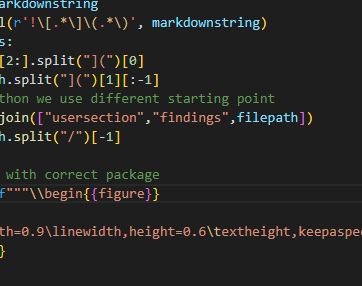
\includegraphics[width=0.9\linewidth,height=0.6\textheight,keepaspectratio=true]{Beispieldateien/images/2022-06-22-23-56-25.png}
	\caption{testimage}
	\label{2022-06-22-23-56-25.png}
\end{figure}
        

\begin{verbatim}
some codeblock
	yep +\_ _ _ \
\end{verbatim}


I tried to create almost public domain sources.
testtest\textit{testtest}.
However, the clarinet sample, some images and the Makefile are (probably) not public domain (see LICENCE file).
Note that the dependencies (ctrulib, sf2d, ...) are NOT in the public domain. Therefore, the binaries wouldn't be, either.

You need to patch issue \url{https://github.com/xerpi/sf2dlib/issues/41} in sf2dlib before compiling the game. In sf2d\_texture.c change TEX\_MIN\_SIZE from 32 to 64.

Changelog :
v0.1.1
	- Makefile supports building cia
	- Updated to work with current sf2d

v0.1
	- Initial Release.
